\documentclass[8.01x]{subfiles}
\begin{document}

\chapter{Midterm 3}

\section{Problem 1: Momentum change}

``A block of mass $m = \SI{2}{kg}$ is initially at rest on a horizontal surface. At time $t = 0$, we begin pushing on it with a horizontal force that varies with time as $F(t)=\beta t^2$, where $\beta = \SI{1.2}{N/s^2}$. We stop pushing at time $t_1 = \SI{5}{s}$. [$F(t) = 0$ for $t>t_1$].

(a) First, assume the surface is frictionless. What is the magnitude of the final momentum of the block at $t_1 = 5$ s? (in kg m/s)''

Since the mass is initially at rest, the final momentum equals the impulse, $\displaystyle p_{fin} = I = \int F(t) dt$.

In other words, we need to solve a simple integral, with a constant coefficient.

\begin{equation}
p_{fin} = \beta \int_0^{t_1} t^2 \mathop{dt} = \beta \Big[ \frac{t^3}{3} \Big]_0^{t_1} = \frac{\beta t_1^3}{3} 
\end{equation}

For $\beta = \SI{1.2}{N/s^2}$ and $t_1 = \SI{5}{s}$, we find $p_{fin} = \SI{50}{kg m/s}$.

``b) Let us now consider a new situation where the object is initially at rest on a rough surface. The coefficient of static friction is $\mu_s = 0.2$. What is the speed of the block at time $t_2 = 5$ s? For simplicity, we take static and kinetic friction coefficients to be the same, $\mu_s = \mu_k$ and consider $g = \SI{10}{m/s^2}$.''

First, let's identify the forces on the block. We have gravity, $m g$, downwards, and a normal force of equal magnitude $N = m g$ upwards, since there is no vertical acceleration.\\
Horizontally, there is the external force $F(t)$ in one direction, and a frictional force $F_f \le \mu_s m g$ in the other. Once the object is moving, $F_f = \mu_k m g$ at all times (since the force never goes below the threshold again).

Before it has started to move, the frictional force equals $F(t)$; this happens until $F(t) > \mu_s m g$, i.e. until the static friction reaches the maximum possible value. When does that happen? Let's see. I will call this time $t_1$, not to be confused with the one used in part (a).

\begin{align}
\beta t_1^2 &= \mu_s m g\\
t_1 &= \sqrt{\frac{\mu_s m g}{\beta}}
\end{align}

The dimension works out correctly (as a sanity check), and $t_1 = \SI{1.825742}{s}$.\\
Again, a check (this is an exam!): $F(1.825742) = 4$ N, while $\mu m g = 4$ N also.

After that time has passed, the object is sliding, and we can find the acceleration by applying Newton's second law. Alternatively, we can find the final momentum using the impulse-momentum theorem, after which we simply divide by the mass to find the speed.\\
Actually, both would involve a time-integral of a force, divided by mass... So I suppose they are very much the same.

The net force is now given by $\beta t^2 - \mu_k m g$. We integrate that from $t_1$ to $t_2$, and divide by the mass $m$.

\begin{align}
v &= \frac{1}{m} \int_{t_1}^{t_2} \beta t^2 \mathop{dt} - \mu_k g \int_{t_1}^{t_2} \mathop{dt}\\
v &= \frac{\beta}{m} \Big[ \frac{t^3}{3} \Big]_{t_1}^{t_2} - \mu_k g (t_2 - t_1)\\
v &= \frac{\beta (t_2^3 - t_1^3)}{3m} - \mu_k g (t_2 - t_1)
\end{align}

With $t_2 = \SI{5}{s}$ and $t_1$ as above we find $v = 17.4343$ m/s.

``(c) What is the power $P$ provided by the force $F(t)$ at time $t_3 = 4$ s (in Watts) in the case where there is friction (part (b))?''

Power is given by $P = \vec{F} \cdot \vec{v} = F v$ (in this case, since the instantaneous force and the instantaneous speed are fully parallel).\\
First, we calculate the velocity at $t = 4$ s using the above formula, and find $v(t=4) = 7.23432$ m/s.\\
Next, we calculate the force at that time: $F(t=4) = \beta (\SI{4}{s})^2 = 19.2 $ N.

Finally, the instantaneous power is the product of the two: $P(t=4) = 138.899$ W.

\section{Problem 2: Torque}

``A uniform solid disc of mass m and radius r is acted upon by three forces of given magnitudes (see the diagram).

\begin{center}
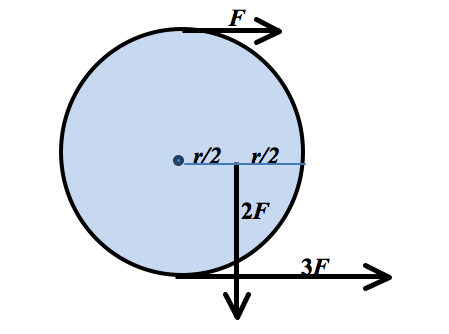
\includegraphics[scale=0.65]{Graphics/midterm3p2}
\end{center}

(a) If the disc rotates about an axis perpendicular to the screen and passing through the center of the disc (as it is viewed from top as in the figure), the magnitude of the angular acceleration, $\alpha$, and the sense of rotation of the disc as viewed from top is:''

\begin{enumerate}
\item $\alpha=2F/(mr)$; counterclockwise
\item $\alpha=2F/(mr)$; clockwise
\item $\alpha=4F/(mr)$; counterclockwise
\item $\alpha=4F/(mr)$; clockwise
\item $\alpha=6F/(mr)$; counterclockwise
\item $\alpha=6F/(mr)$; clockwise
\end{enumerate}

All right, let's see.\\
First, the two forces that act on the edges work against each other, for a net torque of $r(3F - F) = 2 r F$, counterclockwise (out of the screen).\\
The third force is also clockwise, working against the above, with moment arm $r/2$ and force $2F$, for a torque $r F$, clockwise.

The net torque is therefore $r F$, counterclockwise. The moment of inertia for rotation about this axis is $\displaystyle \frac{1}{2} m r^2$. $\tau = I \alpha$, so $\displaystyle \alpha = \frac{\tau}{I}$:

\begin{equation}
\alpha = \frac{r F}{(1/2) m r^2} = \frac{2 F}{m r} \text{ (CCW)}
\end{equation}

``(b) If the disc rotates about an axis perpendicular to the screen and passing through the point of application of force $3F$ (as it is viewed from top as in the figure), the magnitude of the angular acceleration, $\alpha$, and the sense of rotation of the disc as viewed from top is:''

\begin{enumerate}
\item $\alpha=2F/(mr)$; counterclockwise
\item $\alpha=2F/(mr)$; clockwise
\item $\alpha=4F/(mr)$; counterclockwise
\item $\alpha=4F/(mr)$; clockwise
\item $\alpha=6F/(mr)$; counterclockwise
\item $\alpha=6F/(mr)$; clockwise
\end{enumerate}

OK, so first, what is the torque about this point? It's certainly not the same as it was before (and neither is the moment of inertia).\\
The $3F$ force causes no torque through this point. The force at the top is $2r$ away, causing a torque $2 r F$, clockwise.\\
For the third force, we use the fact that the cross product is given by the the magnitude of one vector, times the perpendicular distance of the other. Here, the perpendicular distance of the position vector is $r/2$, so $\tau = (r/2)(2F) = r F$, also clockwise.

Summed together, there is a net torque $3 r F$, clockwise. Next, the moment of inertia. We use the parallel-axis theorem, so the moment of inertia is the same as before, plus $m d^2$ where $d$ is the distance between axes, i.e. $r$ for this problem.

\begin{align}
\alpha = \frac{3 r F}{(1/2) m r^2 + m r^2} = \frac{2 F}{m r} \text{ (CW)}
\end{align}

The rotation is now in the opposite direction, since the only CCW force causes no torque.

``(c) If the disc rotates about an axis perpendicular to the screen and passing through the point of application of force $2F$ (as it is viewed from top as in the figure), the magnitude of the angular acceleration, $\alpha$, and the sense of rotation of the disc as viewed from top is:''

\begin{enumerate}
\item $\alpha=4F/(mr)$; counterclockwise
\item $\alpha=4F/(mr)$; clockwise
\item $\alpha=2F/(mr)$; counterclockwise
\item $\alpha=2F/(mr)$; clockwise
\item $\alpha=8F/(3mr)$; counterclockwise
\item $\alpha=8F/(3mr)$; clockwise
\end{enumerate}

One more time. For a change, let's calculate the moment of inertia first. Again, using the parallel axis theorem: $I = (1/2) m r^2 + m (r/2)^2 = (3/4) m r^2$\\
Next, we calculate the torque. The $2F$ force causes no torque relative to its own application point. The perpendicular distance to the $3F$ force is $r$, so the torque is $3 r F$, direction CCW.\\
The force at the top is has the same perpendicular distance, for a torque of $r F$, direction CW.\\
The net torque is then $2 r F$, CCW, since they work against each other.

\begin{align}
\alpha = \frac{2 r F}{(3/4) m r^2} = \frac{8 F}{3 m r} \text{ (CCW)}
\end{align}

\section{Problem 3: Massive pulley}

\begin{center}
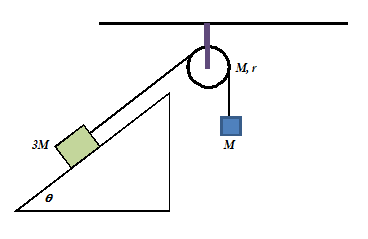
\includegraphics[scale=1.0]{Graphics/midterm3p3}
\end{center}

``In the diagram, block $3M$ slides downward without friction. The string connecting blocks $3M$ and $M$ is ideal (that is, its mass can be neglected and it is not stretchable). The pulley, a uniform solid disc of mass $M$ and radius $r$, rotates without slipping. Find the acceleration of block $3M$.''

\begin{enumerate}
\item $a=(2g/9)(3\cos\theta - 1)$
\item $a=(3g/5)(2\sin\theta + 1)$
\item $a=(g/3)(\sin\theta + 1)$
\item $a=(2g/9)(3\sin\theta - 1)$
\item $a=(3g/5)(2\cos\theta + 1)$
\item $a=(g/3)(\cos\theta + 1)$
\end{enumerate}

Okay. We set up Newton's second law equations for the two blocks, and one of the rotational variants for the pulley, using the no-slip condition, $\displaystyle a = \alpha R \Rightarrow \alpha = \frac{a}{R}$.

Since the $3 M$ block slides downwards, I use that as the position direction, as well as counterclockwise rotation for the pulley.\\
Tension $T_1$ acts on the $3M$ block, while $T_2$ acts on the $M$ block. $T_1 > T_2$, or the pulley would have to rotate in the opposite direction

\begin{align}
3 M g \sin \theta - T_1 &= 3M a\\
T_2 - M g &= M a\\
r(T_1 - T_2) &= (1/2) M r^2 \frac{a}{r}
\end{align}

I will solve this as I usually do: solve the two first equations for $T_1$ and $T_2$ respectively, and then substitute those into the torque equation.

The first:

\begin{align}
3 M g \sin \theta - T_1 &= 3M a\\
T_1 &= 3M (g \sin \theta - a)
\end{align}

The second:
\begin{align}
T_2 - M g &= M a\\
T_2 &= M (a + g)
\end{align}

And the dirty work:

\begin{align}
r(3 M g \sin \theta - 3 M a - (M a + M g)) &= (1/2) M r^2 \frac{a}{r}\\
3 g \sin \theta - 3 a - a - g &= (1/2) a\\
g(3 \sin \theta - 1) &= (9/2) a\\
(2g/9)(3 \sin \theta - 1) &= a\\
\end{align}

\section{Problem 4: Angular collision 2}

\begin{center}
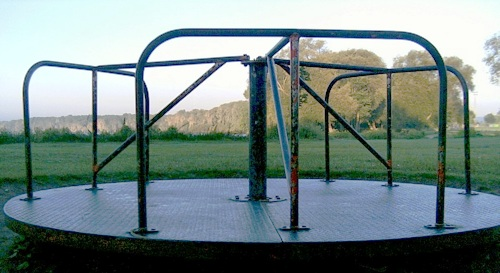
\includegraphics[scale=0.7]{Graphics/midterm3p4}
\end{center}

``A merry-go-round (pictured) is sitting in a playground. It is free to rotate, but is currently stationary. You can model it as a uniform disk of mass 180 kg and radius 130 cm (consider the metal poles to have a negligible mass compared to the merry-go-round). The poles near the edge are 117 cm from the center.

Someone hits one of the poles with a 7 kg sledgehammer moving at 16 m/s in a direction tangent to the edge of the merry-go-round. The hammer is not moving after it hits the merry-go-round.

How much energy $|\Delta E|$ is lost in this collision? (enter a positive number for the absolute value in Joules)''

Alright. The moment of inertia, modeling the merry-go-round as a solid disk, is $(1/2) m r^2 = \SI{152.1}{kg m^2}$. 

The sledgehammer has a linear momentum of $(\SI{7}{kg})(\SI{16}{m/s}) = \SI{112}{kg m/s}$, and a kinetic energy of, using $\displaystyle \frac{1}{2} m v^2$, 896 J. All of the momentum is transferred to the pole, and then to the merry-go-round, causing an angular impulse. All of its kinetic energy is also transferred from it/converted, but not all of it becomes rotational kinetic energy (or the answer to this question would be zero).

The sledgehammer hits a distance 1.17 m from the center, causing an angular impulse $J = (\SI{1.17}{m})(\SI{112}{kg m/s}) = \SI{131.04}{kg m^2/s}$ ($J = \tau \Delta t = r p = r F \Delta t = \Delta L$, so this is also the new angular momentum, relative to the center, since $L_{cm} = 0$ to begin with.)

We can calculate the rotational velocity after the collision using $L_{cm} = I_{cm} \omega \Rightarrow \omega = \frac{L_{cm}}{I_{cm}}$, which is the rotational equivalent to $v = p/m$. Doing that, we find $\omega = 0.86154$ rad/s. The rotational kinetic energy is then

\begin{equation}
E_{post} = \frac{1}{2} I \omega^2 = \SI{56.448}{J}
\end{equation}

So how much energy was lost? Subtracting the initial and final energies, $\Delta E = \SI{896}{J} - \SI{56.448}{J} = \SI{839.552}{J}$ was lost (to heat, vibration, noise, etc).

\section{Problem 5: Ballistic missile}

\begin{center}
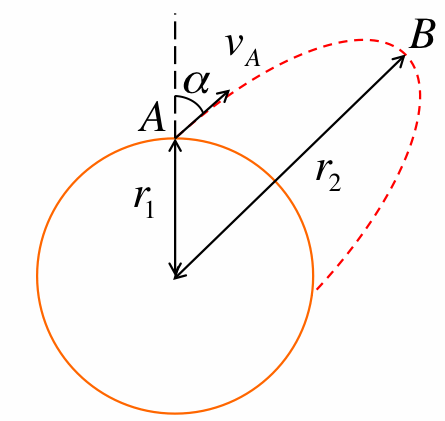
\includegraphics[scale=0.6]{Graphics/midterm3p5}
\end{center}

``A spherical non-rotating planet (with no atmosphere) has mass $m_1 = \SI{4e24}{kg}$ and radius $r_1 = 5000$ km. A projectile of mass $m_2 \ll m_1$ is fired from the surface of the planet at a point A with a speed $v_A$ at an angle $\alpha=\ang{30}$ with respect to the radial direction. In its subsequent trajectory the projectile reaches a maximum altitude at point B on the sketch. The distance from the center of the planet to the point B is $r_2 = (5/2) r_1$. Use $G = \SI{6.674e-11}{kg^{-1} m^3 s^{-2}}$.

What is the initial speed $v_A$ of the projectile? (in m/s)''

(Note: Having looked at the staff solutions after the exam, before I post these notes, I realize that this solution is overly complex. There's no need whatsoever to find $a$, and frankly I should've taken a step back to realize that while solving!)

Okay. The trajectory is clearly part of an ellipse; by the looks of it, a focus could certainly be at the center of the planet. In other words, we can treat this as an elliptical orbit. We enter it at some point (the launch site) with a velocity $v_A$ tangential to the orbit. The total energy of the orbit is the kinetic energy at that point, plus the gravitational potential energy at that point. That must always be equal to $\displaystyle -\frac{G m_1 m_2}{2a}$, where $a$ is the semi-major axis of the orbit.

\begin{align}
\frac{1}{2} m_2 v_A^2 - \frac{G m_1 m_2}{r_1} = -\frac{G m_1 m_2}{2a}
\end{align}

We do know the distance to apogee (at point B): it's given as $r_2 = (5/2) r_1$. The question is: does this imply that the distance from the center of the planet to the other edge of the orbit (perigee) is $r_1$? That is, is the orbit tangent to the planet's surface on the other side, so that $2a = r_1 + r_2$?

Well, we can try to find this out. We can apply both the conservation of mechanical energy and the conservation of angular momentum (about the center of the planet) to the system.\\
First, we use the conservation of mechanical energy at the launch site and at apogee:

\begin{equation}
-\frac{G m_1 m_2}{2a} = \frac{1}{2} m_2 v_B^2 - \frac{G m_1 m_2}{r_2}
\end{equation}

We now have two equations; the unknowns are $v_A$, $a$ and $v_B$. ($r_2$ is known, in terms of $r_1$.)\\
Next, we use the conservation of angular momentum; if we can do so without adding any unknowns, things are looking good. We equate initial angular momentum with that at $B$:

\begin{equation}
r_1 m_2 v_A \sin \alpha = r_2 m_2 v_B
\end{equation}

$\alpha$ is known, so this should now be solvable with quite a bit of work... Collecting the equations with trivial simplifications (cancelling $m_2$, multiplying through by 2 in the top two equations):

\begin{align}
v_A^2 - \frac{2 G m_1}{r_1} &= -\frac{G m_1}{a}\\
-\frac{G m_1}{a} &= v_B^2 - \frac{2 G m_1}{r_2}\\
r_1 v_A \sin \alpha &= r_2 v_B\\
r_2 &= (5/2) r_1
\end{align}

Eliminating $r_2$:

\begin{align}
v_A^2 - \frac{2 G m_1}{r_1} &= -\frac{G m_1}{a}\\
-\frac{G m_1}{a} &= v_B^2 - \frac{2 G m_1}{(5/2) r_1}\\
r_1 v_A \sin \alpha &= (5/2) r_1 v_B\\
\end{align}

We can solve the last equation for $v_B$ in terms of $v_A$:

\begin{equation}
(2/5) v_A \sin \alpha = v_B
\end{equation}

The remaining equations are

\begin{align}
v_A^2 - \frac{2 G m_1}{r_1} &= -\frac{G m_1}{a}\\
-\frac{G m_1}{a} &= ((2/5) v_A \sin \alpha)^2 - \frac{2 G m_1}{(5/2) r_1}\\
\end{align}

Since these equations are equal, we can set the sides containing $v_A$ equal and solve.

\begin{align}
v_A^2 - \frac{2 G m_1}{r_1} &= \frac{4}{25} v_A^2 \sin^2 \alpha - \frac{4 G m_1}{5 r_1}\\
v_A^2 - \frac{4}{25} v_A^2 \sin^2 \alpha &= \frac{2 G m_1}{r_1} - \frac{4 G m_1}{5 r_1}\\
v_A^2 (1 - \frac{4}{25} \sin^2 \alpha) &= \frac{6 G m_1}{5r_1}\\
v_A &= \sqrt{\frac{6 G m_1}{5r_1 (1 - \frac{4}{25} \sin^2 \alpha)}}
\end{align}

8169.46 m/s is the answer then, and $2a \neq r_1 + r_2$. Good thing I didn't assume that; using that leads to an answer more than 5\% too high, so it would most likely have been graded as incorrect (as it should!).

\section{Problem 6: Rocket acceleration}

``Consider a rocket in space that ejects burned fuel at a speed of $v_{ex} = 2.0$ km/s with respect to the rocket. The rocket burns 10\% of its mass in 290 s (assume the burn rate is constant).

(a) What is the speed $v$ of the rocket after a burn time of 145.0 s? (suppose that the rocket starts at rest; and enter your answer in m/s)

(b) What is the instantaneous acceleration a of the rocket at time 145.0 s after the start of the engines? (in $\text{m/s}^2$)''

The definition of thrust (derived from conservation of momentum) is that $F = v_{ex} \frac{dm}{dt}$, only instead $v_{ex}$ I'm used to $u$.\\
We know that $F = m a$, but here, everything is a function of time, including the mass of the rocket.

Instead, we can use conservation of momentum. The derivation for this is shown in lecture.\\
We can show that

\begin{equation}
\Delta v = - v_{ex} \ln \frac{m_f}{m_i}
\end{equation}

(sometimes called the rocket equation) where $\Delta v$ is the change in velocity, $m_f$ the final mass of the rocket, and $m_i$ the initial mass of the rocket; both of the masses include the fuel, of course, or they would be equal.

For part (a), we need simply stick in $m_f/m_i = 0.95$ (since if the burn rate is constant, and it burns 10\% in 290 s, it must burn 5\% in 145 s).

We need to write this in mathematical form later, though, so let's do that now instead. We find

\begin{equation}
m_f/m_i = 1 - 0.1 \frac{t}{\SI{290}{s}}
\end{equation}

Anyway, back to the velocity. Using the above,

\begin{equation}
\Delta v = - v_{ex} \ln \left(  1 - 0.1 \frac{t}{\SI{290}{s}} \right)
\end{equation}

We can simply plug the numbers in. The initial velocity is zero, so that implies that $v = \Delta v$:

\begin{equation}
v = \SI{102.58}{m/s}
\end{equation}

for an average acceleration of $\SI{0.7}{m/s^2}$; rather pathetic, to be honest!

Next is the instantaneous acceleration. We can find this from the above using a bit of calculus. We can take the derivative ``manually'', by finding

\begin{equation}
\frac{\Delta v}{\Delta t} = \frac{v_{t + \Delta t} - v_t}{\Delta t} = \frac{1}{\Delta t}\left( - v_{ex} \ln \left(1 - 0.1 \frac{t + \Delta t}{\SI{290}{s}}\right) + v_{ex} \ln \left(1 - 0.1 \frac{t}{\SI{290}{s}}\right) \right)
\end{equation}

In the limit where $\Delta t \to 0$, this becomes the derivative of the velocity, which of course is the acceleration.\\
At $t = \SI{145}{s}$, this gives us $a = \SI{0.726}{m/s^2}$ or so. Alternatively, we could simply take the derivative the usual way. We have 

\begin{equation}
v = C \ln (u)
\end{equation}
which has the derivative

\begin{equation}
\frac{dv}{dt} = C \frac{1}{u} \frac{du}{dt} = -2000 \left( \frac{1}{1 - 0.1 \frac{t}{\SI{290}{s}}} \right) (-\frac{1}{\SI{2900}{s}})
\end{equation}

Evaluated at $t = \SI{145}{s}$, this also gives us $a = \SI{0.726}{m/s^2}$.

\section{Problem 7: Doppler shift}

``A source of sound emits waves at a frequency $f = 450$ Hz. An observer is located at a distance $d = 160$ m from the source. Use $u = 340$ m/s for the speed of sound.

(a) Assume completely still air. How many wavefronts (full waves) $N$ are there between the source and the observer?

(b) If the observer is moving away from the source at a (radial) velocity $v = 40$ m/s, how does the number of wavefronts $N$ found in part (a) change with time? For the answer, give the rate of change of N, namely $\displaystyle \frac{dN}{dt}$.

(c) By comparing the difference of the rate of wavefronts leaving and wavefronts entering the region between source and observer, calculate the frequency $f′$ observed by the moving observer. (in Hz)\\
hint: how does the difference relate to the rate of change of N you calculated in (b)?

(d) Let us now assume that both source and observer are at rest, but wind blows at a constant speed $v = 20$ m/s in the direction source towards observer. By comparing the difference of the rate of wavefronts leaving and wavefronts entering the region between source and observer, calculate the observed frequency f′? (in Hz)''

First, to get us started, wavelength is given by $\displaystyle \lambda = \frac{u}{f}$. Therefore, the wavelength of 450 Hz sound is $0.75555$ m (with the five repeating).

Part (a) is easy, then: $\displaystyle N = \frac{\SI{160}{m}}{\SI{0.755555}{m}} = 211.765$ wavefronts.\\
I would ordinarily round this down to 211, since the question asks for ``full waves'', but in a clarification on the wiki it was stated no rounding is necessary.

For part (b), it's clear that the number must increase, since the distance is increasing. As the observer is the one moving, there shouldn't be any other effects to consider (if the \emph{source} moves, wavefronts are compressed/spaced out, etc).

The distance is increasing by 40 meters each second; each meter contains a bit more than one wavefront at this frequency, so the answer must be a bit above 40 ($40/0.75555$). Using the chain rule, with $dd/dt$ as the rate of change of distance (since they labeled it $d$),

\begin{equation}
\frac{dN}{dt} = \frac{dd}{dt} \cdot \frac{dN}{dd}
\end{equation}

The first number is given as $40$ m/s, while the second is just the number of wavefronts per meter (the reciprocal of meters per wavefront, i.e. wavelength), so

\begin{equation}
\frac{dN}{dt} = (\SI{40}{m/s})(\frac{1.3235}{\SI{1}{m}}) \approx \SI{52.94}{wavefronts/s} = \SI{52.94}{Hz}
\end{equation}

As intuitively expected, this is just the velocity divided by the wavelength (or, equivalently, multiplied by the wavelength's reciprocal). In terms of symbols,

\begin{equation}
\frac{dN}{dt} = \frac{dd}{dt} \frac{f}{u}
\end{equation}

``(c) By comparing the difference of the rate of wavefronts leaving and wavefronts entering the region between source and observer, calculate the frequency $f′$ observed by the moving observer. (in Hz)\\
hint: how does the difference relate to the rate of change of N you calculated in (b)?''

Interesting! I hadn't realized this relationship, I must say. We find

\begin{align}
f - f' &= \frac{dN}{dt}\\
f' &= f - \frac{dN}{dt}
\end{align}

which I will admit I partly realized this because I knew the formula for Doppler shift to begin with, which gives the same numerical answer.\\
In the case where the observer is moving towards the source, the time derivative turns negative (the number of wavefronts between the two is going down), so in that case $f' > f$, as it should be.

Using this, we find $f' = 397.06$ Hz; $f' < f$ since the observer is moving away.

This equation is really saying that the number of wavefronts that reach the receiver ($f'$) is the number of wavefronts sent out per second, minus the number of wavefronts per second you outrun, I suppose. Of course, they will catch up eventually, unless you move at a speed greater than $u$ away.

I believe that by combining the two equations above, we should be able to find ``the'' formula for Doppler shift of a moving observer:

\begin{align}
f' &= f - f \frac{dd}{dt} \frac{1}{u}\\
f' &= f\left(1 - \frac{v_{rad}}{u}\right)
\end{align}

where $\displaystyle \frac{dd}{dt} = v_{rad} = v \cos \theta$ is the radial velocity. Nice!

Finally, part (d), repeated for simplicity:

''(d) Let us now assume that both source and observer are at rest, but wind blows at a constant speed $v = 20$ m/s in the direction source towards observer. By comparing the difference of the rate of wavefronts leaving and wavefronts entering the region between source and observer, calculate the observed frequency f′? (in Hz)''

Since the waves are pressure fronts in the air, and wind is movement of air, the receiver will clearly receive the sound waves earlier than with no wind. How does the perceived frequency change, though?

Intuitively, I would say it does not change, with the following reasoning: if 450 wavefronts enter per second, and more than 450 exit, where did the rest come from? If more exit than enter, the region would have to run out of wavefronts after a while, which makes no sense at all!\\
If less exit than enter, the air would be crowded by wavefronts, which makes equally little sense.\\
The only sensible answer is that wavelength and frequency are unchanged.\\
I suppose this can be shown in a better way than this, but I leave that for another time (and perhaps for the staff solutions?).

\section{Problem 8: Falling ruler}

\begin{center}
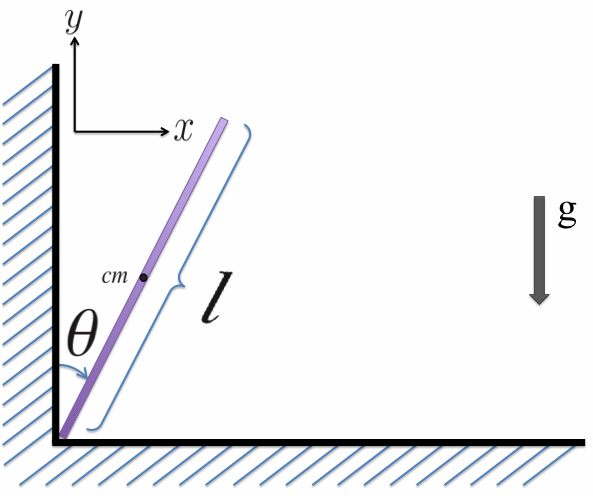
\includegraphics[scale=0.5]{Graphics/midterm3p8}
\end{center}

``A ruler stands vertically against a wall. It is given a tiny impulse at $\theta = \ang{0}$ such that it starts falling down under the influence of gravity. You can consider that the initial angular velocity is very small so that $\omega(\theta=\ang{0})=0$. The ruler has mass $m = 150$ g and length $\ell = 20$ cm. Use $g = \SI{10}{m/s^2}$ for the gravitational acceleration, and the ruler has a uniform mass distribution. Note that there is no friction whatsoever in this problem. (See figure)

(a) What is the angular speed of the ruler $\omega$ when it is at an angle $\theta = \ang{30}$? (in radians/sec)

(b) What is the force exerted by the wall on the ruler when it is at an angle $\theta=\ang{30}$? Express your answer as the $x$ component $F_x$ and the y component $F_y$ (in Newton).

(c) At what angle $\theta_0$ will the falling ruler lose contact with the wall? ($0 \le \theta_0 \le \ang{90}$; in degrees) [hint: the ruler loses contact with the wall when the force exerted by the wall on the ruler vanishes.]''

I've left this problem for last, as I'm a bit confused about exactly what it's asking; the wiki clarifications haven't made it easier, either. It seems to me that $F_y$ for the \emph{wall} (not the floor) should be zero at all times if there is no friction, but that doesn't appear to be the case.\\
One answer also stated that we could treat the entire L-shaped object as the ``wall'' (i.e. wall+floor).

Anyway, it looks to be like this... For part (b), we ignore the wording ``wall'' and simply calculate the contact force, ignoring exactly which structure provides it. (I find it a bit confusing that the wall can provide the vertical force if we consider the ruler 1-dimensional, but apparently that is the case.)\\
For part (c), we find where the contact force from the \emph{vertical wall}, i.e. $F_x$, is zero. $F_y$ will still be greater than zero when that happens. And for part (a), this discussion is not very relevant.

All right, let's get started. Step one: forces. $F_x$ and $F_y$, the total contact force, act in the corner, on the very bottom of the rod.\\
$m g$ acts on the center of mass, a length $\ell/2$ up along the rod.\\
Only gravity can cause a torque relative to the corner; this torque is given by $\tau = (\ell/2) m g \sin \theta$.

To begin with, this torque is zero, and the stick is in equilibrium. When hit with the tiny (negligible, except that it sets the stick in motion) impulse, $\theta$ grows to a tiny angle, and so there is a tiny torque, which is changing with time.

The angular acceleration is given by $\alpha = \tau/I$, so

\begin{equation}
\alpha = \frac{d^2 \theta}{dt^2} = \frac{d \omega}{dt} = \frac{(\ell/2) m g \sin \theta}{I_Q}
\end{equation}

where $I_Q$ is the moment of inertia about that point in the corner, which I choose to label Q.

The moment of inertia is $(1/3) m \ell^2$ for a rod about its end like this; it is found using the moment of inertia about a rod's center of mass $(1/12) m \ell^2$, plus $m (\ell/2)^2$ via the parallel axis theorem. The angular acceleration is therefore given by

\begin{equation}
\alpha = \frac{3 g \sin \theta}{2 \ell}
\end{equation}

where $\theta$ is a function of time. $\alpha = \ddot{\theta}$, so

\begin{equation}
\ddot{\theta} - \frac{3 g}{2 \ell} \sin \theta = 0 
\end{equation}

Hmm. I don't think this is the intended way to solve this. Let's try an energy approach instead. The stick begins with a total energy of $U = m g (\ell/2)$. As it falls, this is converted into rotational kinetic energy. (All of it, assuming we consider about the contact point, and only before it loses contact.)

As it rotates/falls, the center of mass is lowered down, so that it loses potential energy. The height of the center of mass is given by $h = (\ell/2) \cos \theta$.

\begin{align}
m g (\ell/2) &= m g (\ell/2) \cos \theta + \frac{1}{2} I_Q \omega^2\\
m g (\ell/2) &= m g (\ell/2) \cos \theta + \frac{1}{2} \left(\frac{1}{3} m \ell^2\right) \omega^2\\
g (1/2) &= g (1/2) \cos \theta + \frac{1}{6} \ell \omega^2\\
g \left( \frac{1}{2} - \frac{1}{2} \cos \theta\right) &= \frac{1}{6} \ell \omega^2\\
\sqrt{\frac{3 g}{\ell} \left( 1 - \cos \theta\right)} &= \omega
\end{align}

A-ha, much more reasonable.\\
At $\theta = \ang{30}$, we find $\omega = 4.48288$ rad/s.

``(b) What is the force exerted by the wall on the ruler when it is at an angle $\theta=\ang{30}$? Express your answer as the $x$ component $F_x$ and the y component $F_y$ (in Newton).''

I got really, really, really stuck on this one. In fact, I spent most of Sunday and Monday trying to figure out where the heck I was going wrong; I found that $F_x$ vanishes (next question) at 90 degrees. Apparently, it loses contact with the wall earlier, but I couldn't find out how to put that into mathematical terms, even if I understood that it happened.

Below is a solution that is highly inspired by the staff's solution (though all text etc is my own). My alternative solution, which I finally solved the day \emph{after} the exam deadline, follows after that.

\subsection{Staff solution-inspired answers for parts b/c/d}

All forces can be thought of as acting on the center of mass, as far as linear motion is concerned. However, that the center of mass moves towards the right doesn't imply that the end loses contact with the corner; the CoM moves with full contact, to begin with. The ruler couldn't tip over without this initial force (and acceleration), since the center of mass must move towards the right when the ruler tips over.

The center of mass also moves downwards. When these two motions are ``balanced'', so to speak, and the center of mass traces out an arc (i.e. part of a circle, so that it undergoes circular motion), there is still contact, and $F_x > 0$.

In order to find the forces, we use Newton's second law:

\begin{align}
m a_x &= F_x\\
m a_y &= F_y - m g
\end{align}

So we need to find the linear acceleration (of the center of mass).

From work above, we already have

\begin{align}
\omega &= \dot{\theta} = \sqrt{\frac{3g}{\ell} (1 - \cos \theta)}\\
\alpha &= \ddot{\theta} = \frac{3 g}{2 \ell} \sin \theta
\end{align}

Using basic trigonometry, we can find that $x_{cm} = (\ell/2) \sin \theta$ and $y_{cm} = (\ell/2) \cos \theta$. We then take the time derivative of those, twice each, using the chain rule (since $\theta$ is a function of time, and we most certainly can't differentiate with respect to $\theta$ to find the acceleration).

For the second differentiation, we need to use both the product rule and the chain rule.

\begin{align}
v_x &= \frac{d x_{cm}}{dt} = (\ell/2) (\cos \theta) \dot{\theta}\\
a_x &= \frac{d v_x}{dt}    = (\ell/2) (-\sin (\theta) \dot {\theta}^2 + \cos (\theta) \ddot{\theta})
\end{align}

Here, we could either save ourselves some trouble by calculating values for $\omega = \dot{\theta}$ and $\alpha = \ddot{\theta}$ and sticking them in, or find full expressions in terms of the given variables by substituting them in. If we choose the latter, we get, after simplification,

\begin{equation}
a_x = \frac{3}{4} g (3 \cos \theta - 2) \sin \theta
\end{equation}

Multiply this by $m$, since we found that $m a_x = F_x$, and

\begin{equation}
F_x = \frac{3}{4} m g (3 \cos \theta - 2) \sin \theta
\end{equation}

At $\theta = \ang{30}$, this gives us 0.336 N.

We then take a step back and do the same thing for the $y$ component.

\begin{align}
v_y &= \frac{d y_{cm}}{dt} = (\ell/2) (-\sin \theta) \dot{\theta}\\
a_y &= \frac{d v_y}{dt}    = (\ell/2) ((-\cos \theta) \dot{\theta}^2 - (\sin \theta) \ddot{\theta})
\end{align}

Again, we could substitute in values, or do the algebra. In terms of the given variables, and simplified,

\begin{equation}
a_y = -\frac{3}{2} g(1 + 3\cos \theta) \sin^2(\theta/2)
\end{equation}

We can't simply multiply by $m$ to find the force, though: $m a_y = F_y - m g$, so $F_y = m (a_y - g)$.

\begin{equation}
F_y = m\left(g -\frac{3}{2} g(1 + 3\cos \theta) \sin^2(\theta/2)\right)
\end{equation}

which gives us $F_y = 0.957693$ N.

Finally, to find the angle where it loses contact with the wall, we set $F_x = 0$ (as hinted). We can divide away lots of stuff from both sides, which is the nice thing about zero:

\begin{align}
0 &= \frac{3}{4} m g (3 \cos \theta - 2) \sin \theta\\
0 &= 3 \cos \theta - 2\\
\frac{2}{3} &= \cos \theta\\
\arccos \frac{2}{3} &= \theta \approx \ang{48.1897}
\end{align}

This exact angle was the answer to question 5 on exam 5 (``Sliding down a dome''), too, for when a block sliding of a spherical dome loses contact.

\subsection{My own solution}

I'm writing this section the day after the exam, after having realized why my first ``solution'' was incorrect. In short, I tried to find the linear acceleration of the center of mass using $\vec{a} = \vec{\alpha} \times \vec{R}$; however, that equation gives the \emph{tangential acceleration only}.\\
My second attempt was to consider the centripetal acceleration (i.e. the radial acceleration), but I never considered the large picture, and so it was only today, the day after the exam closed, that I realized that these equations only give the respective component, and that they are not two different ways to find the net center of mass acceleration... Any time I get stuck like this, if I try to ``re-start'' the problem, I just end up with the same train of thought again, which is rather frustrating!\\
Anyway, with no further ado... What I wish I'd found a day earlier:

$a_{tan} = \alpha R$, where in this case, $R = \ell/2$.

\begin{equation}
a_{tan} = \frac{\ell}{2} \frac{3 g}{2 \ell} \sin \theta = \frac{3 g}{4} \sin \theta
\end{equation}

Next, we need to find the radial acceleration, i.e. the inwards (towards the corner) centripetal acceleration, which must equal $(\ell/2) \omega^2$ in magnitude, or the center of mass will not undergo circular motion.

\begin{equation}
a_{rad} = (\ell/2) \omega^2 = \frac{3 g}{2} (1 - \cos \theta)
\end{equation}

The net acceleration of the center of mass is the sum of these, but we care about the $x$ and $y$ components rather than their sum, so we take the $x$ and $y$ components of the above accelerations and sum them together, like this:

\begin{align}
a_x &= a_{tan} \cos \theta - a_{rad} \sin \theta\\
    &= \frac{3 g}{4} \sin \theta \cos \theta - \frac{3 g}{2} (1 - \cos \theta) \sin \theta\\
    &= \frac{3 g}{4} \left(\sin \theta \cos \theta - 2 \sin \theta (1 - \cos \theta) \right)
\end{align}

The tangential component is positive (it points towards the right to begin with, and $\hat{x}$ is towards the right), while the radial is negative ($a_{rad}$ points towards the corner, opposite the $x$ axis).

We can find the $y$ component(s) similarly.

\begin{align}
a_y &= -a_{tan} \sin \theta - a_{rad} \cos \theta\\
a_y &= -\frac{3 g}{4} \sin \theta \sin \theta - \frac{3 g}{2} (1 - \cos \theta) \cos \theta\\
a_y &= -\frac{3 g}{4} \left(\sin^2 \theta + 2\cos \theta (1 - \cos \theta)\right)\\
a_y &= -\frac{3 g}{4} \left(\sin^2 \theta + 2(\cos \theta - \cos^2 \theta)\right)
\end{align}

Here, both components are negative; the tangential acceleration starts to the right, and then points down, while $+y$ is up; the radial points down to begin with (the component is always purely down, of course), and is also negative for that reason.

Now that we know these, we can apply the equations we found earlier relating these to the forces we seek. Solved for the forces, they are 

\begin{align}
m a_x &= F_x\\
m a_y + m g &= F_y
\end{align}

So if we make the substitutions,

\begin{align}
\frac{3 m g}{4} \left(\sin \theta \cos \theta - 2 \sin \theta (1 - \cos \theta) \right) &= F_x\\
m g - \frac{3 m g}{4} \left(\sin^2 \theta + 2(\cos \theta - \cos^2 \theta)\right) &= F_y
\end{align}

which gives us, in numbers: $F_x = 0.3364$ N and $F_y = 0.9577$ N.

Finally, to find the angle at where it loses contact with the wall, we set $F_x = 0$ and solve. Lots of stuff can be divided away from both sides as a first step.

\begin{align}
0 &= \frac{3 m g}{4} \left(\sin \theta \cos \theta - 2 \sin \theta (1 - \cos \theta) \right)\\
0 &= \cos \theta - 2 (1 - \cos \theta)\\
2 &= 3\cos \theta\\
\arccos \frac{2}{3} &= \theta
\end{align}

$\theta \approx \ang{48.19}$ is the angle when it loses contact with the wall, and the center of mass stops undergoing circular motion.

Incredibly, this is independent of both the stick's length \emph{and} mass.

\section{Problem 9: Yoyo}

\begin{center}
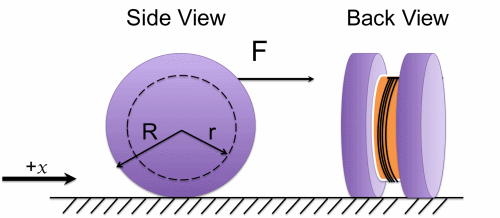
\includegraphics[scale=1.2]{Graphics/midterm3p9}
\end{center}

``A yoyo of mass $m = 2$ kg and moment of inertia $I_{cm} = \SI{0.09}{kg m^2}$ consists of two solid disks of radius $R = 0.3$ m, connected by a central spindle of radius $r = 0.225$ m and negligible mass. A light string is coiled around the central spindle. The yoyo is placed upright on a flat rough surface and the string is pulled with a horizontal force $F = 24$ N, and the yoyo rolls without slipping.

(a) What is the x-component of the acceleration of the center of mass of the yoyo? (in $\text{m/s}^2$)\\
(b) What is the x-component of the friction force? (in N)''

The horizontal force causes a clockwise torque. I will assume the string is wound such that the force is applied at the top, as drawn, even though it's not actually specified in text. (If it were at the bottom, the torque would be in the other direction.)

Here comes the slightly dangerous part... The frictional force is \emph{not} towards the left. For this reason, $a > F/m$ (where $F$ is the pulling force). However, we don't need to know this in advance (I didn't), so let's set up the equation as if friction is towards the left.

With this in mind, writing an equation for the linear acceleration is very easy:

\begin{equation}
F - F_f = m a
\end{equation}

Next, we look at torques. The pull of the string provides a torque $r F$, clockwise.\\
Friction provides a torque $R F_f$, also clockwise, assuming it is towards the left.

$\tau_{cm} = I_{cm} \alpha$; we can use the no-slip condition $\alpha = a/R$ (the part in contact with the ground). We can not use it for the string, however. Less string will be unrolled than what would happen at pure roll at the central spindle.

Our second equation then becomes, using clockwise torque/rotation as positive:

\begin{equation}
\frac{r F + R F_f}{I_{cm}} = \frac{a}{R}
\end{equation}

From the first equation, we find

\begin{equation}
\frac{F - F_f}{m} = a
\end{equation}

Substituted into the second, and using $I_{cm} = 2(\frac{1}{2} \frac{m}{2} R^2$, which cleans things up a bit:

\begin{align}
\frac{r F + R F_f}{I_{cm}} &= \frac{1}{R} \frac{F - F_f}{m}\\
\frac{r F + R F_f}{2(1/2)(m/2) R^2} &= \frac{1}{R m} (F - F_f)\\
\frac{r F + R F_f}{(1/2) R} &= F - F_f\\
\frac{2 r F}{R} - F &= - 3 F_f\\
F\left(1 - \frac{2 r}{R}\right) &= 3 F_f\\
\frac{F}{3}\left(1 - \frac{2 r}{R}\right) &= F_f
\end{align}

In terms of numbers, $F_f = -4$ N. Since it is negative, it is towards the right -- opposite of the assumption.

Finding $a$ is then trivial, using the above equation for $a$. The total force towards the right is 28 N, $m$ is 2 kg, and so $a = \SI{14}{m/s^2}$.

\end{document}